\section{Final Project}
\label{final-project}

In this part of the report, I will explain the project I developed in detail. I will divide the project into two parts: Back-end and Front-end.

For the final project, we were given some time to develop. We were first given time to develop after the \texttt{Spring} framework part. It was for developing the back-end. The second time given was after the \texttt{React} part, which was finished on the second day of the fourth week. Since the main internship program was four weeks at OBSS, we were expected to finish the final project by the end of the fourth week. However, I could not complete the project at this time. Since my internship period was six weeks and I could not complete the project, they asked me to complete the project within this period.

In the fifth week of my internship, I decided to start from scratch because I thought that I made mistakes at many points while developing the project and that if I continued to develop on these mistakes, it would harm the development phase. First, I tried to find out where I lacked and made mistakes.

I tried to learn \texttt{React} from the beginning for three days because I thought I had problems with the \texttt{React} part. As a result of this work, I have come to a position where I can do many things on \texttt{React} without difficulty. I spent the next two days thinking about simple things and design. In my last week, I rebuilt and coded the entire project, starting from scratch.

\subsection{Project and Requirements}

The final project was a basic Book Portal whose requirements were provided. We were provided the \hyperref[book-portal]{document located in the appendicies} for basic requirements.

In my project, there are two main entities: User and Book. Each user has a role, admin or user role, and book lists for favorite and read books. Each book has many information about itself: name, author, type, publisher, and publication date. Both admins and users can log in to the system. Each admin is also a user and can do everything a user can, such as updating passwords, seeing books, adding books to their read or favorite lists, and searching for a book and its information. Additionally, an admin can add, update, and delete users and books.

\subsection{Back-end}

As mentioned in the requirements, I used \texttt{Spring} for the back-end. The main folder structure can be seen \hyperref[back-end-tree]{at the appendicies}. \texttt{Spring Security} is active, and \texttt{JWT} tokens, which need to be inside the request's header, are used for authentication. After security is passed, the request is handled by controllers. In the back-end part, there are nine main folders:
\begin{itemize}
  \item \texttt{config}: contains the configurations and data loader.
  \item \texttt{controller}: contains request (Rest) controllers. If the requests are authorized, they are met by the related controller. When a request is met, necessary business logic is run.
  \item \texttt{entity}: contains entity classes. These entity classes are used in the tables of the database.
  \item \texttt{exception}: contains the user-defined exceptions and global exception handler.
  \item \texttt{filter}: contains filter classes. All requests go through the filters.
  \item \texttt{model}: contains model classes. These classes are used for data transfer between client, server, and database.
  \item \texttt{repo}: contains repositories. These interfaces are used to access the database by using \texttt{Spring JPA}.
  \item \texttt{service}: contains services. These classes consist of the business layer functions.
  \item \texttt{util}: contains utilities.
\end{itemize}
These are the main folders consisting of several files, and I will briefly explain them. These back-end files are accesible in the GitHub repository of this report: \href{https://github.com/burakmetehan/internship-report-2022}{\textbf{Link}}.
\newpage


\subsubsection{\texttt{config}}

The classes inside this folder are used for the configuration of \texttt{Spring} and data loading when \texttt{Spring} runs the app. After the app starts running, the data loader is not used, although configurations influence the app's answer.

\begin{figure}[ht]
  \label{back-end-config-tree}
  \centering
  \begin{forest}
    pic dir tree,
    where level=0{}{
      directory,
    },
    [config
      [AuthEntryPoint.java, file]
      [DataLoader.java, file]
      [PasswordConfig.java, file]
      [WebSecurityConfig.java, file]
    ]
  \end{forest}
  \caption{Structure of config folder.}
\end{figure}

\paragraph{\texttt{AuthEntryPoint.java:}} When authorization is failed in \texttt{Spring Security}, the function inside this class is called and returns a response with the \texttt{UNAUTHORIZED} status code.

\paragraph{\texttt{PasswordConfig.java:}} This class indicates the password encoder which is used through the app.

\paragraph{\texttt{WebSecurityConfig.java:}} It is configuration of \texttt{Spring Web Security} that checks all the requests for authorization and roles. Also, if an exception occurs, it handles the exception with the help of a global exception handler. 

The web security is a little bit confusing and not easy to handle. Especially, \texttt{JWT} token-based authentication challenged me. I spent almost one day understanding what \texttt{JWT} token and \texttt{JWT} token-based authentication are. By reading documents and examining examples, I implemented \texttt{JWT} token-based authentication for my security.

\paragraph{\texttt{DataLoader.java:}} This class is run when the application is run. It checks the database for the default admin user and roles, called \texttt{ROLE\_ADMIN} and \texttt{ROLE\_USER}. If the database is missing, it creates admin user and roles. After learning the \texttt{ApplicationRunner} interface, it was easy to implement.


\subsubsection{\texttt{controller}}

Controllers are the essential elements of back-end development. Controller files are used with \texttt{@RestController} annotation, which indicates that the class is a Rest API controller. Each class has \texttt{@RequestMapping} annotation that shows the path of the controller; that is, the requests coming to the specified path are handled by that class.

The classes include several mappings for different request types such as \texttt{GET}, \texttt{POST}, \texttt{PUT}, or \texttt{DELETE}. When a request is sent to the back-end, \texttt{Spring} sends it to a suitable controller according to \texttt{@RequestMapping}. When a request arrives at the class, it handles it according to its type.

Since controllers are not tricky, I could easily code and map the requests. The most challenging part of the controllers was the authentication of functions. Since some operations, such as deleting users or books, cannot be done by regular users but admins, I needed to secure the related functions. After researching, I managed to block the regular user using some operations by using \texttt{@Secured} annotation. This annotation takes a string which is the privileged role, in my case \texttt{ROLE\_ADMIN}. When this annotation is used, \texttt{Spring Security} checks for the additional role.

\begin{figure}[ht]
  \label{back-end-controller-tree}
  \centering
  \begin{forest}
    pic dir tree,
    where level=0{}{
      directory,
    },
    [controller
      [AuthController.java, file]
      [BookController.java, file]
      [BookListController.java, file]
      [UserController.java, file]
    ]
  \end{forest}
  \caption{Structure of controller folder.}
\end{figure}

\paragraph{\texttt{AuthController.java:}} This class handles the requests coming to the path `\texttt{/auth}' and has two \texttt{POST} mapping.

This class is responsible for authentication operations. It can be used to check the \texttt{JWT} token's validity or log in. Using the information inside the request body, I checked the necessary information and sent the response to the client. The responses include some required information for the front-end, such as validation information, admin status, or \texttt{JWT} token.

\paragraph{\texttt{BookController.java:}} This class handles the requests coming to the path `\texttt{/books}'. It has six \texttt{GET}, one \texttt{POST}, one \texttt{PUT}, and one \texttt{DELETE} mapping. 

This class handles book operations such as searching, adding, updating, or deleting. I need a particular concern in this class: \texttt{Pageable} and \texttt{List} data. Since I needed pageable and list data in the front-end while searching the book, I coded two variances of each search function. This class can handle both id and name searches. In name searches, there is no need to provide the full name of the book. Instead, providing a letter or word inside the book name is enough.

\paragraph{\texttt{BookListController.java:}} This class handles the requests coming to the path `\texttt{/}' and has two \texttt{PUT}. Although the main path is `\texttt{/}', the two functions inside this class have special path mapping for its \texttt{PUT} mapping. This class is responsible for the favorite and read list operations. 

According to the traditional way, updating something is done with \texttt{PUT} request. Since adding or removing a book from read or favorite lists is updating the list, I decided to use \texttt{PUT} requests. However, there were four operations: adding or removing from the read list and adding or removing from the favorite list. Therefore, I decided to have two main functions and paths for read and favorite lists. In main paths `\texttt{/read}' and `\texttt{/fav}', I handled read and favorite list operations, respectively. A request parameter is needed as well as the book and user ids to acquire the necessary information, which book will be added or removed.

\paragraph{\texttt{UserController.java:}} This class handles the requests coming to the path `\texttt{/users}'. It has six \texttt{GET}, one \texttt{POST}, one \texttt{PUT}, and one \texttt{DELETE} mapping.

This class is similar to the book controller and is responsible for user operations such as searching, adding, updating, or deleting. Like in the book controller, I also need a particular concern, \texttt{Pageable} and \texttt{List} data, and I solve this problem the same way in the book controller.


\subsubsection{\texttt{entity}}

Entities are my main data classes. Thanks to \texttt{Hibernate}, I was also able to create the database tables by using \texttt{@Table} annotations, so the tables were created automatically. Around the back-end, such as between data and business layers, I used these entity classes; however, I used models while sharing and transmitting information between the client and server.

The main problem with entity classes was the mutual data types. A \texttt{User} includes \texttt{Set<Book>} inside it, and a \texttt{Book} includes \texttt{Set<User>} inside it. This was a problem when this information was sent to the client side due to this mutuality. For example, when a \texttt{User} is sent to the client, its read list is also sent. However, inside the read list, there are books that contain the \texttt{User} that is being sent to the client. Therefore, there was an infinite loop while parsing the data. I solved it by using \texttt{@ManyToMany}, and \texttt{@JsonManagedReference} annotations.

\begin{figure}[ht]
  \label{back-end-entity-tree}
  \centering
  \begin{forest}
    pic dir tree,
    where level=0{}{
      directory,
    },
    [entity
      [Book.java, file]
      [EntityBase.java, file]
      [Role.java, file]
      [User.java, file]
    ]
  \end{forest}
  \caption{Structure of entity folder.}
\end{figure}

\paragraph{\texttt{Book.java:}} This is an entity class that extends \texttt{EntityBase} for a \texttt{Book} and is responsible for holding information of a book. It has `name', `author', `page count', `type', `publisher', and `publication date' fields as well as the data fields in \texttt{EntityBase}. Also, it has many-to-many relations with \texttt{User} class. 

\paragraph{\texttt{User.java:}} This is an entity class that extends \texttt{EntityBase} for a \texttt{User} and is responsible for holding information of an user. It has `username', `password', `read list', `favorite list', and `roles' fields as well as the data fields in \texttt{EntityBase}. Also, it has many-to-many relations with \texttt{Book} and \texttt{Role} classes. 

\paragraph{\texttt{Role.java:}} This is an entity class that extends \texttt{EntityBase} for a \texttt{User} and is responsible for holding information of a role. It has the `name' field and the data fields in \texttt{EntityBase}. Also, it has many-to-many relations with \texttt{User} class. 

\paragraph{\texttt{EntityBase.java:}} This is an entity class that is the base of other entities. This holds the general information such as `id', `creation date', `update date', or `activity'.


\subsubsection{\texttt{exception}}

Exceptions are used at several points to provide information to the exception handler. The exception handler catches the exceptions and sends a response to the client. The primary purpose of the exception handler is security because default \texttt{Spring} errors exploit some system information. Therefore, I used special exceptions and an exception handler to provide necessary but unimportant information outside.

Creating new exception classes was not hard. However, adjusting the exception handler is a little tough because the order of the functions can be a problem. I solved this problem using \texttt{@Order} annotations and attention.

\begin{figure}[ht]
  \label{back-end-exception-tree}
  \centering
  \begin{forest}
    pic dir tree,
    where level=0{}{% folder icons by default; override using file for file icons
      directory,
    },
    [exception
      [BadRequestException.java, file]
      [BookListException.java, file]
      [BookNotFoundException.java, file]
      [ConflictException.java, file]
      [GlobalExceptionHandler.java, file]
      [RoleNotFoundException.java, file]
      [UserNotFoundException.java, file]
    ]
  \end{forest}
  \caption{Structure of exception folder.}
\end{figure}

The names of the files explain what the classes are for and what they do. These are used for specified exceptions in related positions.


\subsubsection{\texttt{filter}}

My app contains only one filter, which is checking the \texttt{JWT} token. I use \texttt{JWT} token for authentication purpose because transmitting username and password in all request is hard and can cause security vulnerabilities. If the \texttt{JWT} token does not exist in the header or it is expired, \texttt{BadRequestException} is thrown, and a response is returned with \texttt{BAD\_REQUEST} status code.

This part challenged me because I did not know \texttt{JWT} and how to check it, and I spent almost one day for this authentication system. However, the main problem was not that the subject was difficult but that I misunderstood some concepts and topics and needed to change the security configuration quite a bit.

\begin{figure}[ht]
  \label{back-end-filter-tree}
  \centering
  \begin{forest}
    pic dir tree,
    where level=0{}{
      directory,
    },
    [filter
      [JwtRequestFilter.java, file]
    ]
  \end{forest}
  \caption{Structure of filter folder.}
\end{figure}


\subsubsection{\texttt{model}}

Models are mainly used to transmit data between client and server sides. There were two reasons. The first one is that client does not know some information, such as the creation date while the latter is that the client should not need to see some information, such as the user's password or the object's update date. Therefore, I used DTOs for any information transfer between the client and server sides.

One class, called \texttt{MyUserDetails}, is not used for information transfer. It was needed for the authentication system. It helps by indicating how the necessary information is extracted from the \texttt{User} entity.

\begin{figure}[ht]
  \label{back-end-model-tree}
  \centering
  \begin{forest}
    pic dir tree,
    where level=0{}{
      directory,
    },
    [model
      [AuthDTO.java, file]
      [AuthResponseDTO.java, file]
      [BookDTO.java, file]
      [BookResponseDTO.java, file]
      [BookUpdateDTO.java, file]
      [JwtRequest.java, file]
      [JwtResponse.java, file]
      [MyUserDetails.java, file]
      [RoleResponseDTO.java, file]
      [UserDTO.java, file]
      [UserResponseDTO.java, file]
      [UserUpdateDTO.java, file]
    ]
  \end{forest}
  \caption{Structure of model folder.}
\end{figure}


\subsubsection{\texttt{repo}}

Repositories are used to access the databases, and they make use of the \texttt{Spring JPA} by extending \texttt{JpaRepository}. Some essential operation, such as directly adding or finding by id, is inside the \texttt{JpaRepository} but if I want to add something special, I write the function name by using keywords, such as \texttt{findBy}, or \texttt{All}, and \texttt{Spring} generates the necessary queries in the background. This is so easy to use and increases the speed of development.

\begin{figure}[ht]
  \label{back-end-repo-tree}
  \centering
  \begin{forest}
    pic dir tree,
    where level=0{}{
      directory,
    },
    [repo
      [BookRepository.java, file]
      [RoleRepository.java, file]
      [UserRepository.java, file]
    ]
  \end{forest}
  \caption{Structure of repo folder.}
\end{figure}

There is one for each main entity. \texttt{BookRepository} is used for operations on books, \texttt{UserRepository} is used for operations on users, and \texttt{RoleRepository} is used for operations on roles.


\subsubsection{\texttt{service}}

Services are the business layer of my app. All the operations, such as adding or removing the books or users, and logic are done in this layer. Controllers use the services for related operations; therefore, it can be said that there is one service for each controller.

Inside services, other services or necessary repositories are used. Accessing the database is done inside services with the help of repositories that contain several different implementations of the same operation for different needs. For example, several search functions exist for pageable and list data.

\begin{figure}[ht]
  \label{back-end-service-tree}
  \centering
  \begin{forest}
    pic dir tree,
    where level=0{}{
      directory,
    },
    [service
      [BookListService.java, file]
      [BookService.java, file]
      [JwtUserDetailsService.java, file]
      [UserService.java, file]
    ]
  \end{forest}
  \caption{Structure of service folder.}
\end{figure}
\newpage


\subsubsection{\texttt{util}}

This folder contains only one class, called \texttt{JwtTokenUtil}. This class contains several functions applicable to the \texttt{JWT} token, such as getting the username or expiration date from the token. Also, it can generate a new \texttt{JWT} token. \texttt{JWT} filter and \texttt{AuthController} excessively used this class.

\begin{figure}[ht]
  \label{back-end-util-tree}
  \centering
  \begin{forest}
    pic dir tree,
    where level=0{}{
      directory,
    },
    [util
      [JwtTokenUtil.java, file]
    ]
  \end{forest}
  \caption{Structure of util folder.}
\end{figure}


\newpage
\section{Front-end}

As mentioned the requirements, I used React for front-end. The main folder structure can be seen at the appendicies \hyperref[front-end-tree]{front-end-tree}. I used \textbf{antd}, which is an enterprise-class UI design language and React UI library, for user interface, Node.js, which is a JavaScript runtime built on Chrome's V8 JavaScript engine, and npm, packages manager.

In the front-end part, there are 2 main folders: public and src. The folder public contains the default \texttt{public.html} when npm is used to create the project and \texttt{public.html} contains only one div whose id is `\texttt{root}' and which will be modified through entire app. 

\subsection{Folder Structure}

The main project files are inside the src folder.
\begin{itemize}
  \item \texttt{globals}: It is a folder and contains the global variables of the app.
  \item \texttt{pages}: It is a folder and contains the pages, called auth, book, and user, as well as the main homepage of the app.
  \item \texttt{service}: It is a folder and contains the service layer of front-end. Files inside this folder include functions to connect the back-end.
  \item \texttt{App.js}: It is a file and responsible for rendering the pages and providing the main/top navigations around the app. Also, it checks the authorization token and its validation.
  \item \texttt{index.js}: It is a file and responsible for rendering \texttt{App.js} by using \texttt{ReactDOM}.
\end{itemize}

I will briefly explains the folder and files in detail. Then I will tell the pages.

\subsubsection{\texttt{globals}}

This folder contains just a file, called \texttt{GlobalVariables}. That file contains two global variables, called \texttt{BOOK\_COLUMNS} and \texttt{PAGINATION} which are used for tables around app.

\begin{figure}[ht]
  \centering
  \begin{forest}
    pic dir tree,
    where level=0{}{% folder icons by default; override using file for file icons
      directory,
    },
    [\dots
      [globals
        [GlobalVariables.js, file]
      ]
    ]
  \end{forest}
  \caption{Structue of globals}
\end{figure}

\subsubsection{\texttt{pages}}

This folder contains the whole pages, which means users mainly see the files inside this folder. I will explain the pages in details later.

\begin{figure}[ht]
  \centering
  \begin{forest}
    pic dir tree,
    where level=0{}{% folder icons by default; override using file for file icons
      directory,
    },
    [\dots
      [pages
        [auth
          [\dots, file]
        ]
        [book
          [\dots]
        ]
        [user
          [\dots]
        ]
        [Home.js, file]
      ]
    ]
  \end{forest}
  \caption{Structue of pages}
\end{figure}

\paragraph{\texttt{Home.js}:}

This is the homepage of the app and contains the general information of the user. It can be accessed by clicking the \texttt{Home} from the top navigation.

\paragraph{\texttt{auth}:}

This folder contains just a file, called \texttt{Login}, and it is responsible for login page.

\paragraph{\texttt{book}:}

This is the page of books. It contains five folders and one file inside it, and is responsible for the operations adding, deleting, updating and adding/remove books to/from favorite/read lists. It uses switch for rendering the right page of the operaiton.

\paragraph{\texttt{user}:}

This is the page of users. It contains four folders and one file inside it, and is responsible for the operations adding, deleting, updating. It uses switch for rendering the right page of the operaiton.

\subsubsection{\texttt{service}}

This folder contains the services to access the back-end. The functions inside the service files handle the returned response and return new object with the data inside response. Additionally, thanks to axios interceptor, authorization token, which is saved to \texttt{Session Storage} or \texttt{Local Storage} while logging in, is added the header of all requests.

\begin{figure}[ht]
  \centering
  \begin{forest}
    pic dir tree,
    where level=0{}{% folder icons by default; override using file for file icons
      directory,
    },
    [\dots
      [service
        [AuthService.js, file]
        [BookListService.js, file]
        [BookService.js, file]
        [UserService.js, file]
      ]
    ]
  \end{forest}
  \caption{Structue of service}
\end{figure}

\begin{itemize}
  \item \texttt{AuthService}: Responsible for authentication and login process.
  \item \texttt{BookListService}: Responsible for adding/removing books to/from read/favorite lists.
  \item \texttt{BookService}: Responsible for book operations such as searching, adding, removing and updating.
  \item \texttt{UserService}: Responsible for user operations such as searching, adding, removing and updating.
\end{itemize}

\subsection{Pages}

When the app is run, firstly \texttt{index.js} renders the \texttt{App.js}. \texttt{App.js} firstly checks the authorization token and its validation. If the token is valid, it directs user to the homepage, rendering (\texttt{Home.js}). If the token is not valid, it directs user to the login page, rendering (\texttt{Login.js}).

\subsection{Login and Logout}

This page contains basic login form. While login page is done by antd form, logout item is constructed by `Popconfirm' of antd. If the `\texttt{Remember me}' option is chosen, auhorization token is saved into both \texttt{Session Storage} and \texttt{Local Storage}. However, if it is not chosen, the token is only saved into \texttt{Session Storage}.

\begin{minipage}{.49\textwidth}  
  \begin{figure}[H]
    \centering
  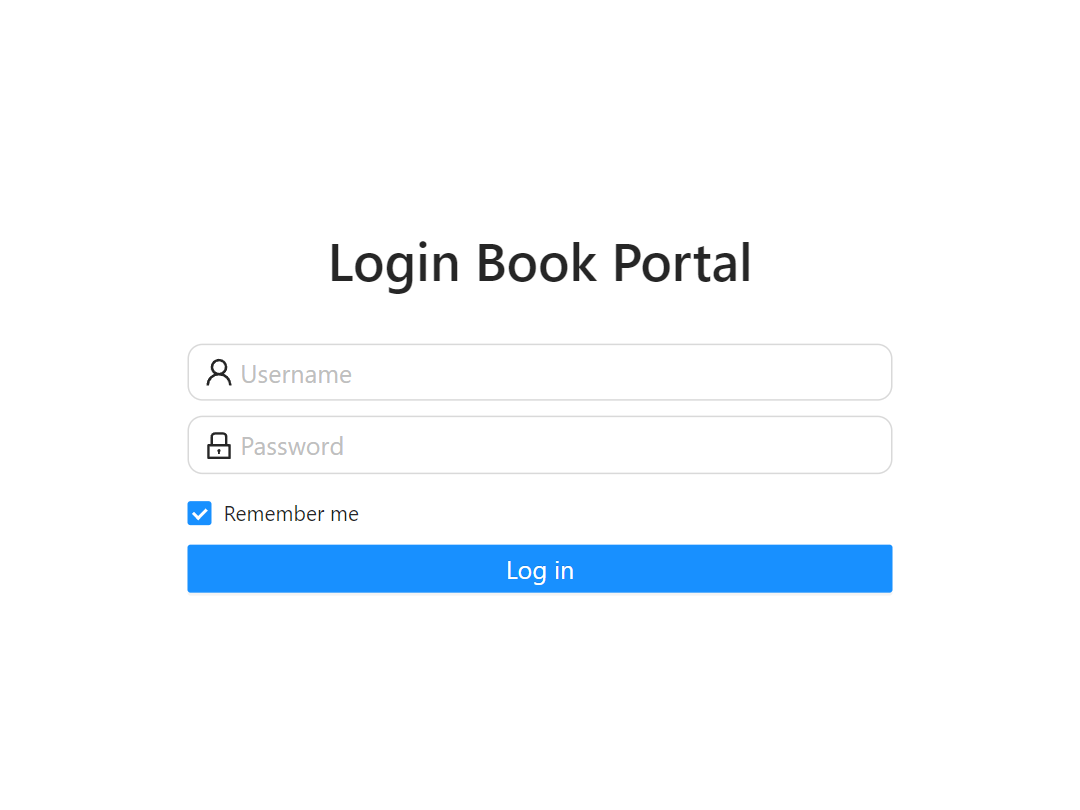
\includegraphics[width=\textwidth]{img/front-end/login-page.png}
  \caption{Login Page}
  \end{figure}
\end{minipage}
\begin{minipage}{.49\textwidth}
  \begin{figure}[H]
    \centering
  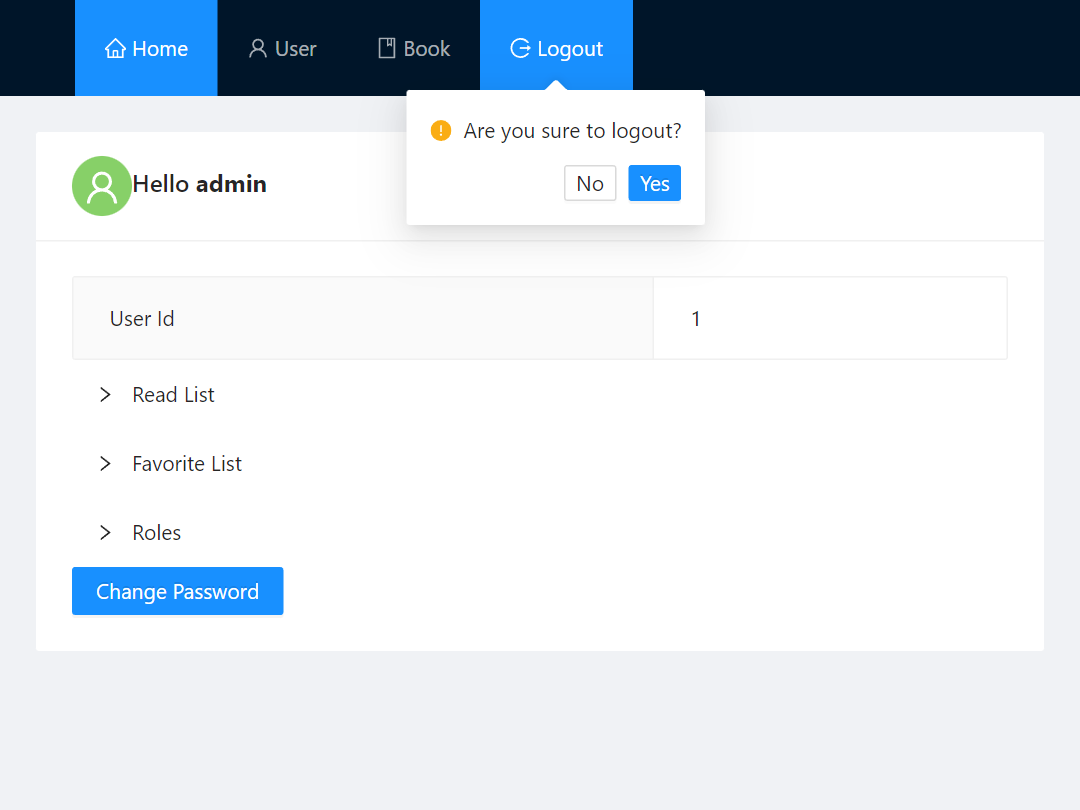
\includegraphics[width=\textwidth]{img/front-end/logout.png}
  \caption{Logout}
  \end{figure}
\end{minipage}

% \begin{figure}[ht]
%   \centering
%   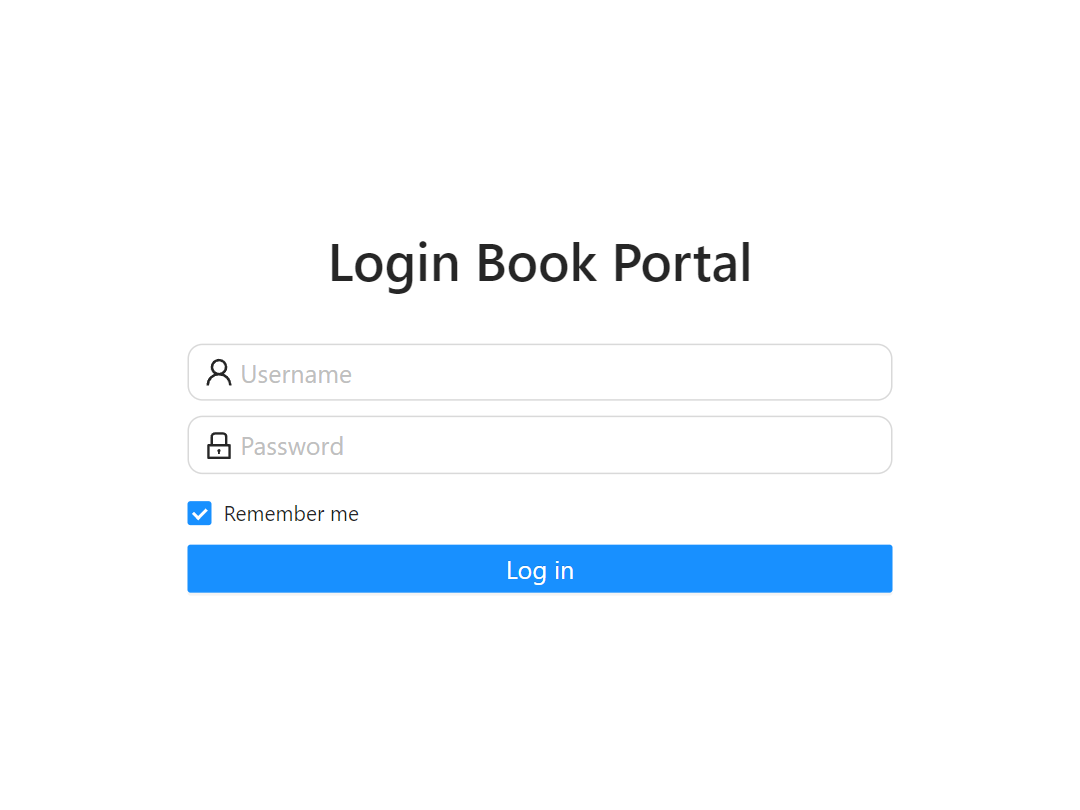
\includegraphics[width=\textwidth]{img/front-end/login-page.png}
%   \caption{Login Page}
% \end{figure}

After logging in, users are directed to homepage. At the top of the screen, there are four different menu items, called \texttt{Home}, \texttt{User}, \texttt{Book} and \texttt{Logout}. Home is firstly rendering and by using these navigations page can be changed. When users clicked to \texttt{Logout}, a warning, which asks users whether they are sure to logout, popped up that. If yes is clicked, users are directed to login page.

% \begin{figure}[ht]
%   \centering
%   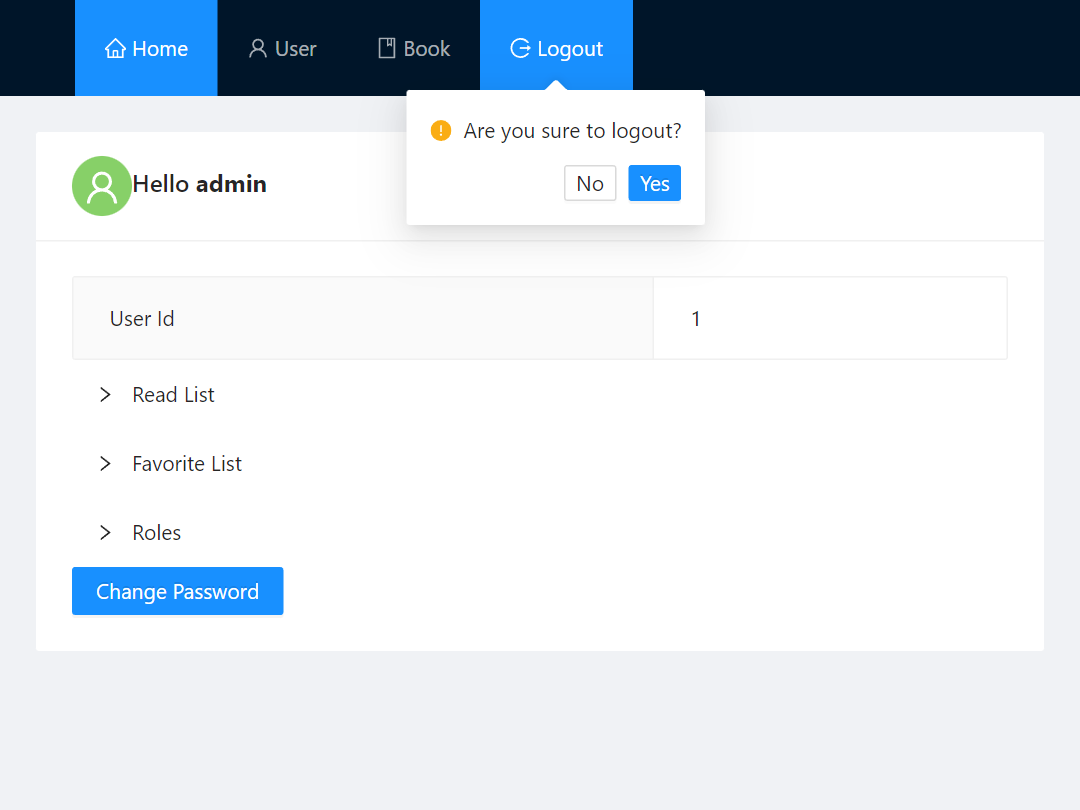
\includegraphics[width=\textwidth]{img/front-end/logout.png}
%   \caption{Logout}
% \end{figure}

\subsection{Home}

In the homepage, user information is provided. This page makes use of `Card', `Descriptions', `Collapse', and `Panel' of antd to show the information. Users can see their user ids, read lists, favorite lists, and roles in this screen. These information is acqiured by sending back-end a request by username and setting information state. By using the button ``Change Password'', they can also access update form and change their passwords.

\begin{minipage}{.49\textwidth}  
  \begin{figure}[H]
    \centering
    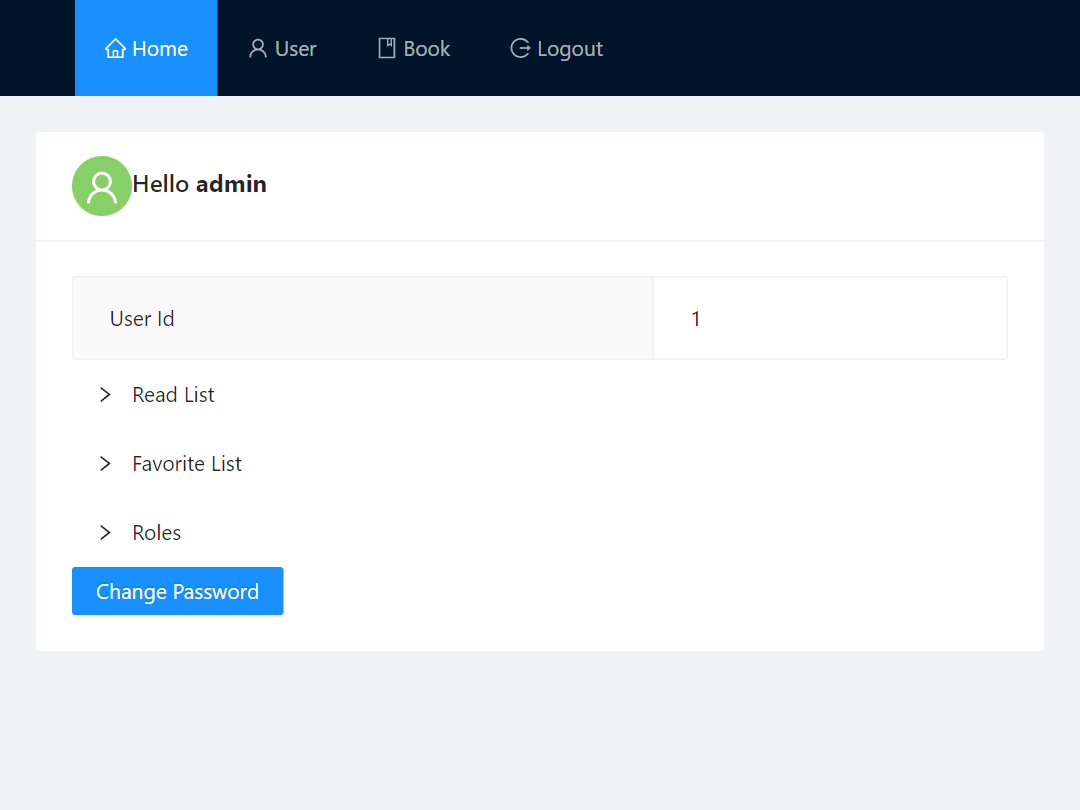
\includegraphics[width=\linewidth]{img/front-end/homepage.png}
    \caption{Home Page}
  \end{figure}
\end{minipage}
\begin{minipage}{.49\textwidth}
  \begin{figure}[H]
    \centering
    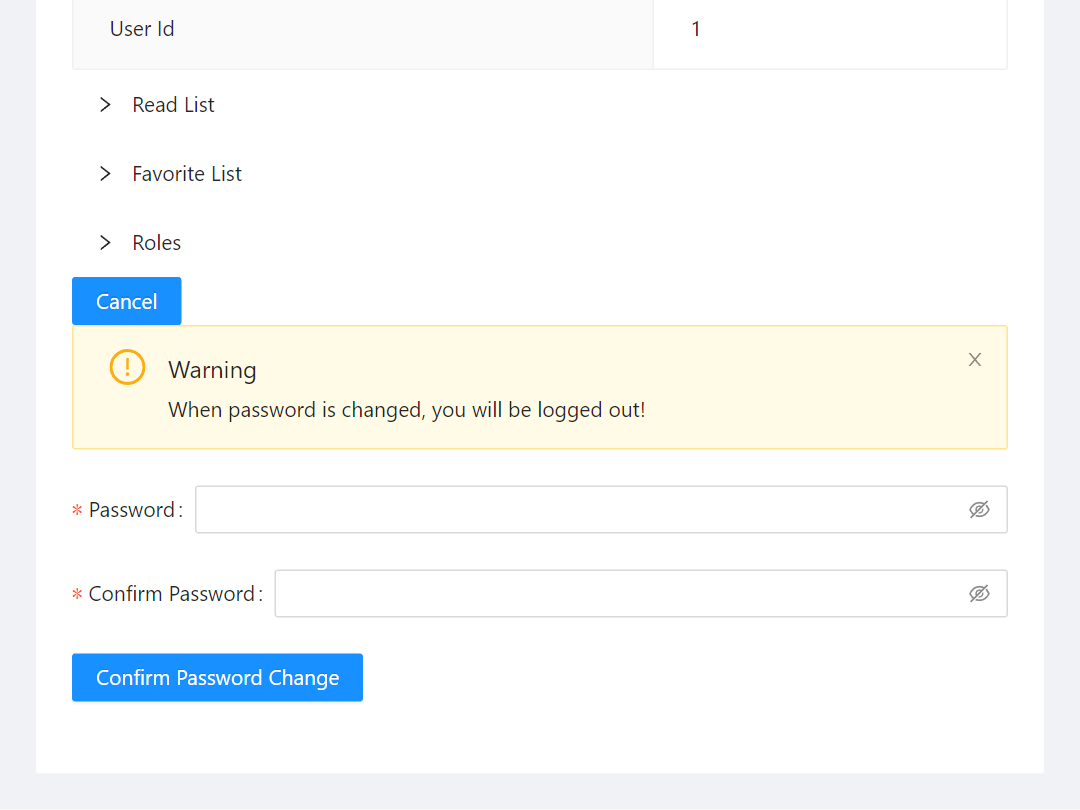
\includegraphics[width=\textwidth]{img/front-end/homepage-password.png}
    \caption{Password Change}
  \end{figure}
\end{minipage}

Since normal users are not allowed to do user operations such as adding, deleting, or updating, \texttt{User} page is special to admins. Therefore, \texttt{User} item is not seen when the user does not have admin roles.

\begin{figure}[H]
  \centering
  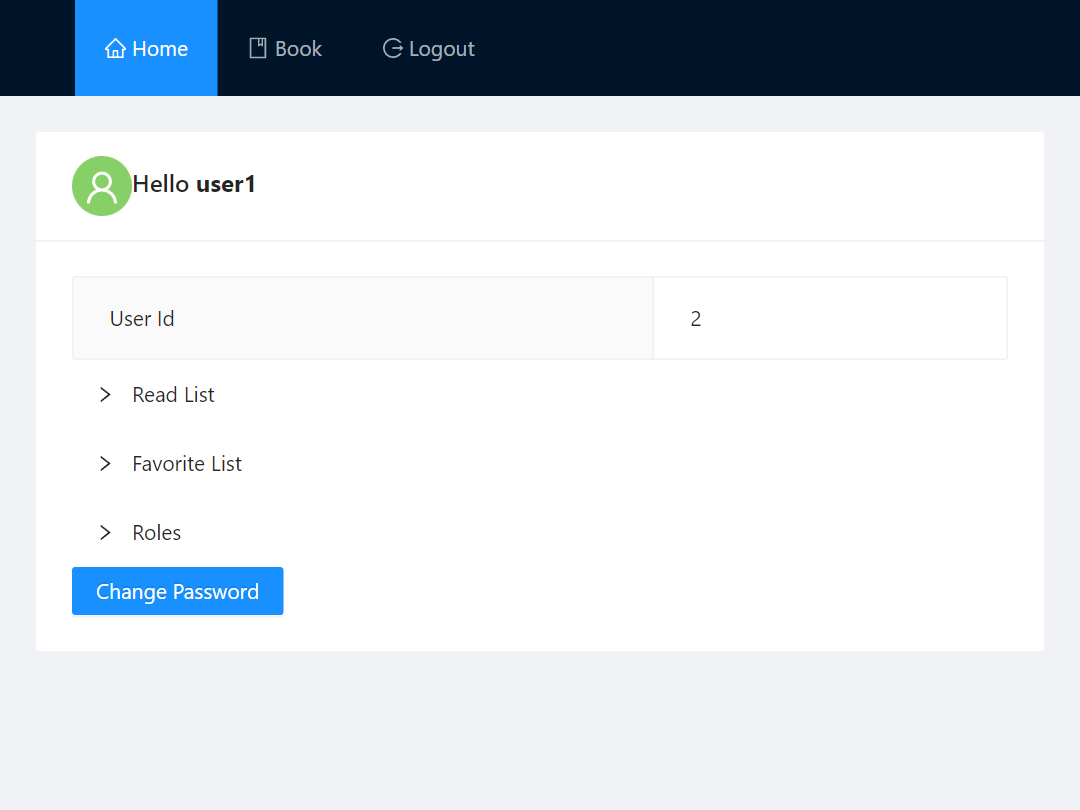
\includegraphics[width=\textwidth]{img/front-end/homepage-user.png}
  \caption{User Home Page}
\end{figure}


\subsection{User}

When \texttt{User} is clicked form top navigaiton, \texttt{User} page is rendered. In this page there are three operations: adding, deleting and updating users. By default \texttt{Add User} is rendered. This page is special to admins because users are not allowed to add, delete, or update users. Therefore, this page is only accessible when the user does not have admin role.

\begin{figure}[H]
  \centering
  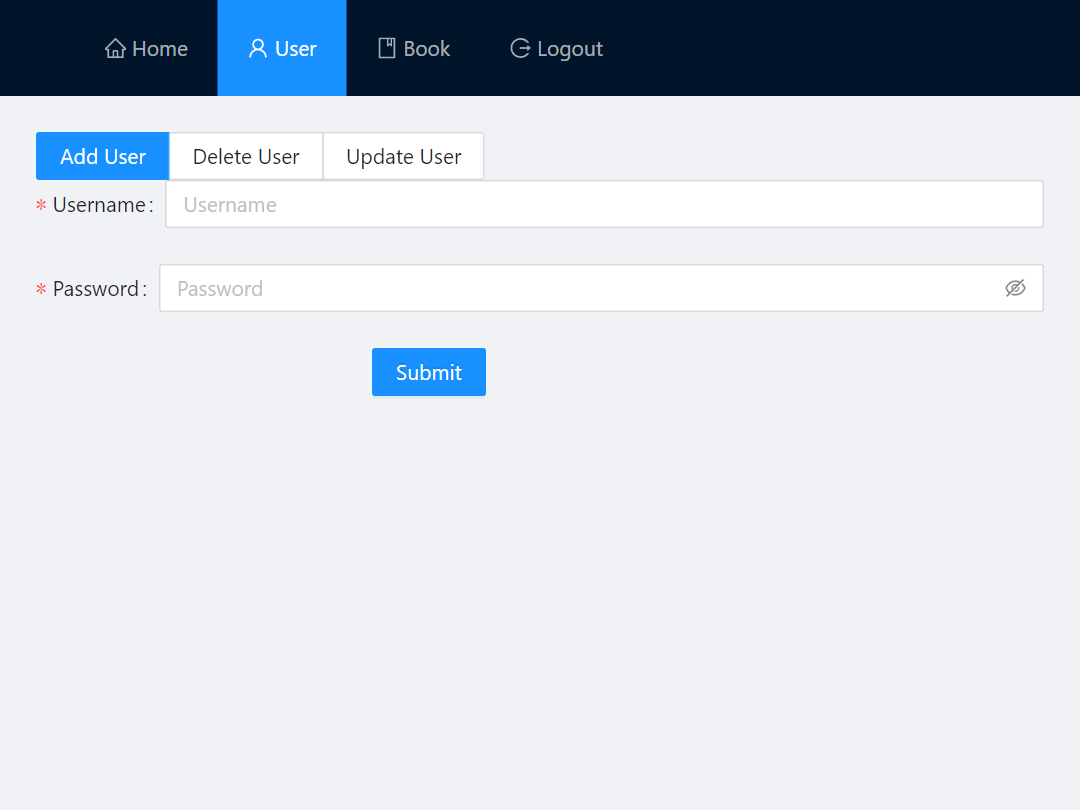
\includegraphics[width=\textwidth]{img/front-end/user.png}
  \caption{User Page}
\end{figure}

\texttt{Add User} contains a basic antd form while \texttt{Delete User} and \texttt{Update User} contains more advanced components. When \texttt{Delete User} and \texttt{Update User} are firstly rendered, a request is sent to database to acquire users and their information by using \texttt{useEffect} of React. These pages also utilize pagination and utilities located in util folder of user.

\texttt{Delete User} and \texttt{Update User} are pretty similar to each other. Both pages support searching users by both id and username, and searching option can be changed by using the radio buttons. When id or username is provided and clicked the search button, a request is sent to back-end through \texttt{UserService}. When the input area is cleared, page is updated and user data is resetted. Both pages also support the pagination and pagination setting changes. Admin can change the pagination setting by using the navigation below. When pagination is changed, a new request is sent to back-end. Additionally, in both pages, admin can see the information of the users.

\begin{minipage}{.49\textwidth}
  \begin{figure}[H]
    \centering
    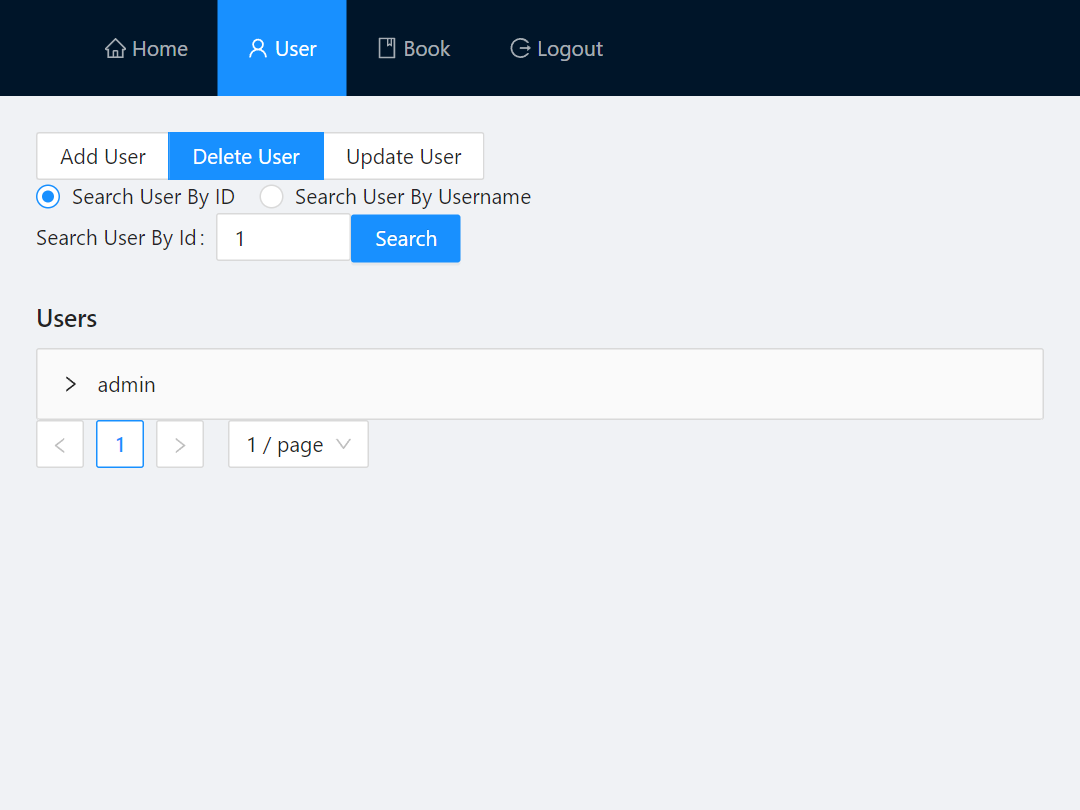
\includegraphics[width=\linewidth]{img/front-end/user-delete-id-search.png}
    \caption{Searching by ID}
  \end{figure}
\end{minipage}
\begin{minipage}{.49\textwidth}
  \begin{figure}[H]
    \centering
    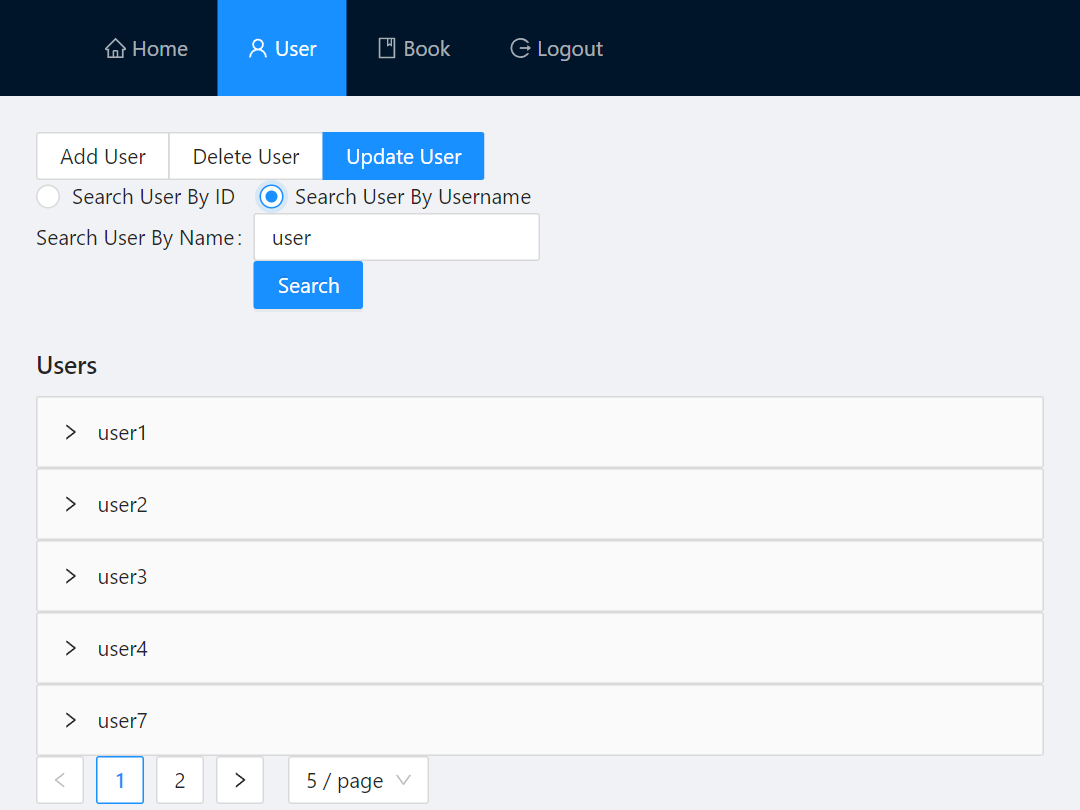
\includegraphics[width=\linewidth]{img/front-end/user-update-name-search.png}
    \caption{Searching by Name}
  \end{figure}
\end{minipage}

Pagination and visualizing the data was the most hard part for me because there were several aspects I need to consider. I changed my visualizing method third times for convenience of developing. Because of this reason, I had to change back-end at some points, so I lost so much time for visualizing decision. However, after visualizing decision is done, my job is not done because pagination is a little bit harder than I expected. Since I misunderstood some parts and concepts of pagination and its callback functions, I had to spent a couple of hours to search and read the antd documentation. In the end, I understood what I should do.

The difference between \texttt{Delete User} and \texttt{Update User} is the buttons found in all users. In \texttt{Delete User}, name of button is `Delete User' and it is used for deleting the user. In \texttt{Update User}, name of button is `Update User' and when it is clicked password update form is appeared.

\begin{minipage}{.49\textwidth}
  \begin{figure}[H]
    \centering
    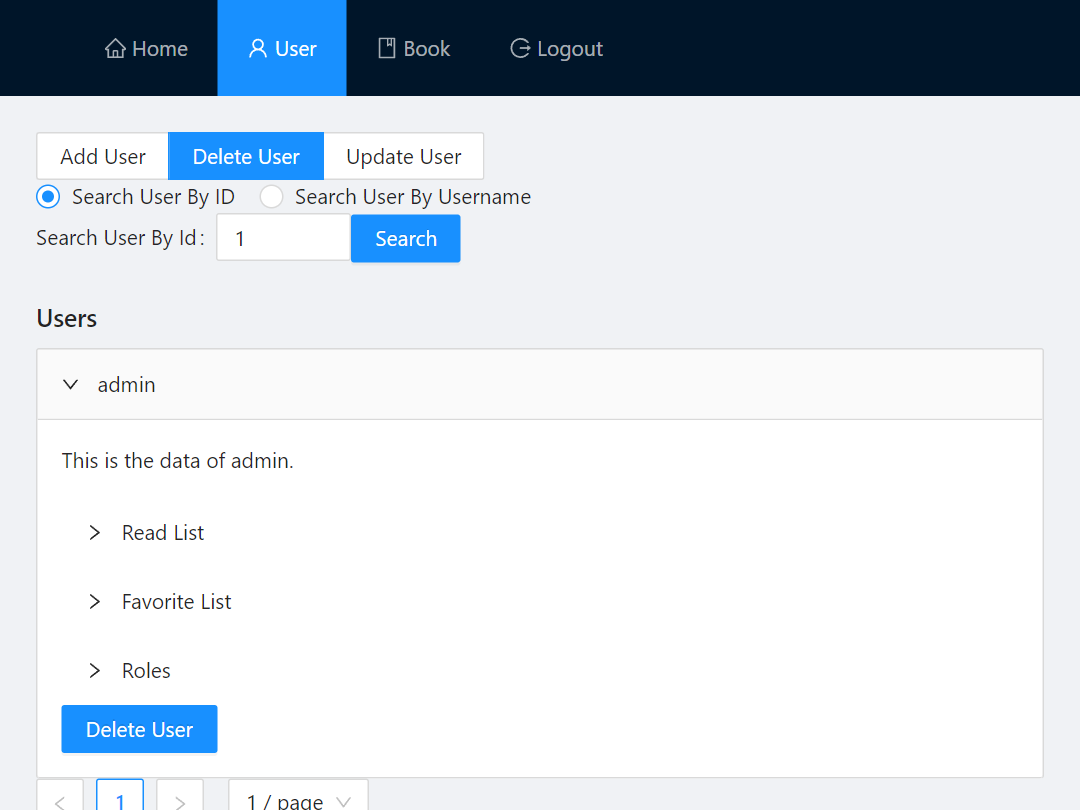
\includegraphics[width=\linewidth]{img/front-end/user-delete.png}
    \caption{Delete User}
  \end{figure}
\end{minipage}
\begin{minipage}{.49\textwidth}
  \begin{figure}[H]
    \centering
    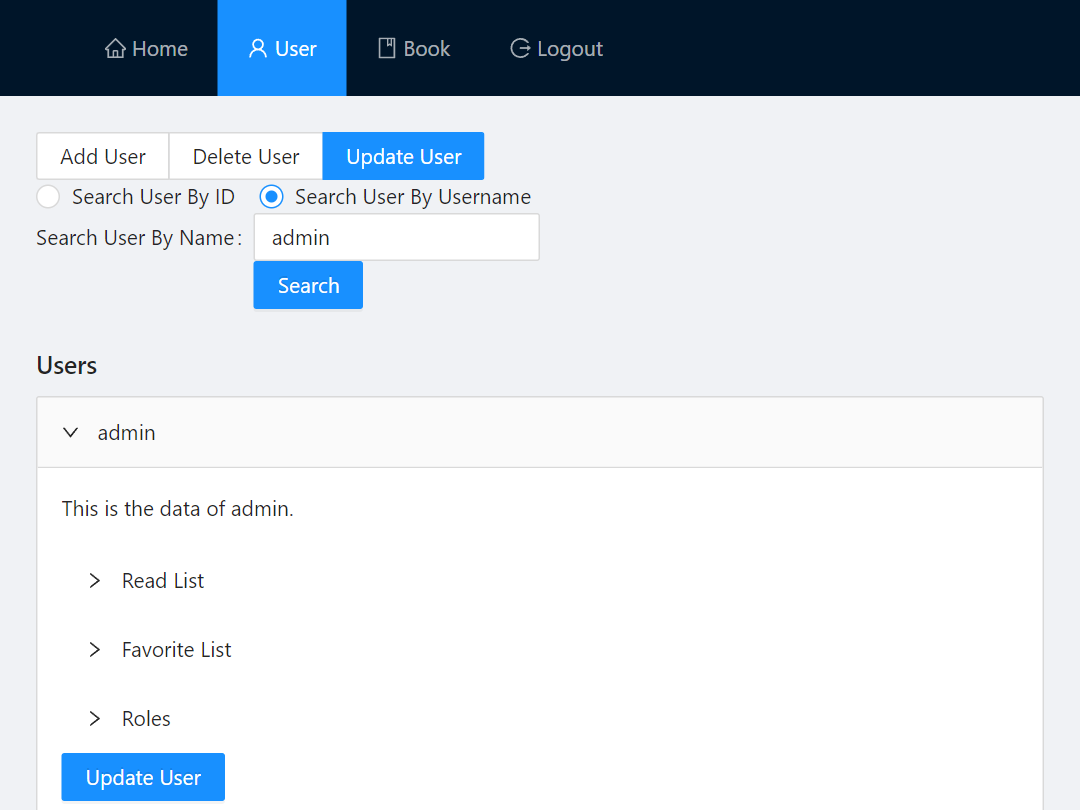
\includegraphics[width=\linewidth]{img/front-end/user-update.png}
    \caption{Update User}
  \end{figure}
\end{minipage}

\subsection{Book}

When \texttt{Book} is clicked form top navigaiton, \texttt{Book} page is rendered. In this page there are three operations: adding, deleting, updating, and listing books. By default \texttt{Book List} is rendered. Although this page is not special, some operations are not allowed to normal users. Therefore; normal users are just allowed listing books and adding/removing these books to/from their lists.

\begin{minipage}{.49\textwidth}
  \begin{figure}[H]
    \centering
    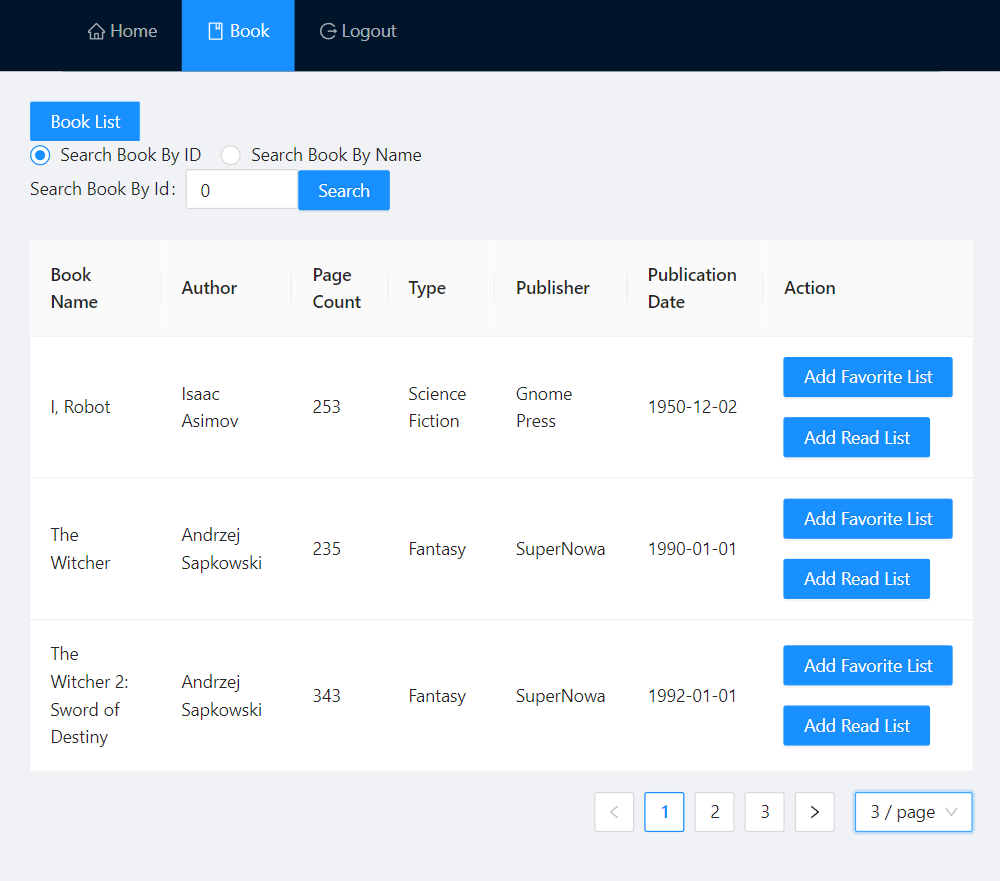
\includegraphics[width=\linewidth]{img/front-end/book-no-admin.png}
    \caption{Book Page for Normal User}
  \end{figure}
\end{minipage}
\begin{minipage}{.49\textwidth}
  \begin{figure}[H]
    \centering
    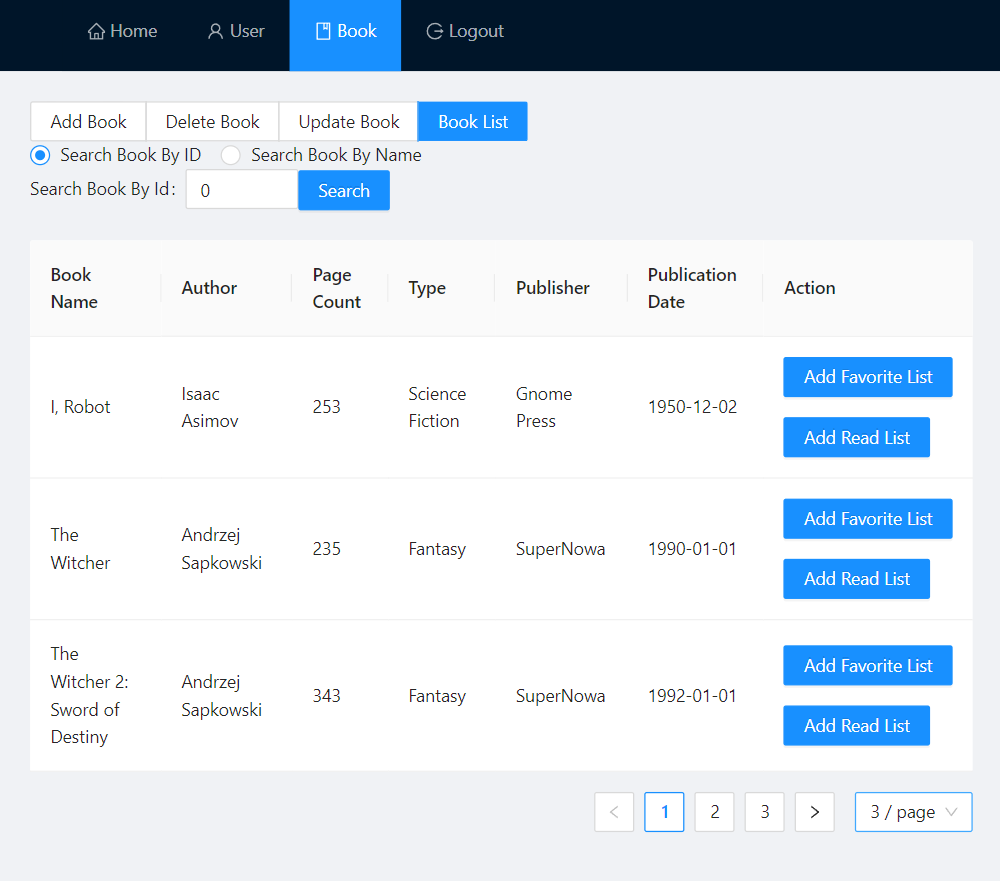
\includegraphics[width=\linewidth]{img/front-end/book-admin.png}
    \caption{Book Page for Admins}
  \end{figure}
\end{minipage}

\subsubsection{\texttt{Add Book}}

This page is for adding book to database and special to admins. When the option is chosen, \texttt{Add Book} is rendered and provides a form to add book. The fields of \texttt{Book} entity: name, author, page count, type, publisher and publication date. All the fields are required and the date can be chosen from calendar. When the book is submitted, a request is sent to back-end to save the book by the help of \texttt{BookService}. When book is saved, the information of the saved book is shown below of the form. Additionally, the size of the form can be changed by using the `Form Size' radio buttons.

\begin{minipage}{.49\textwidth}
  \begin{figure}[H]
    \centering
    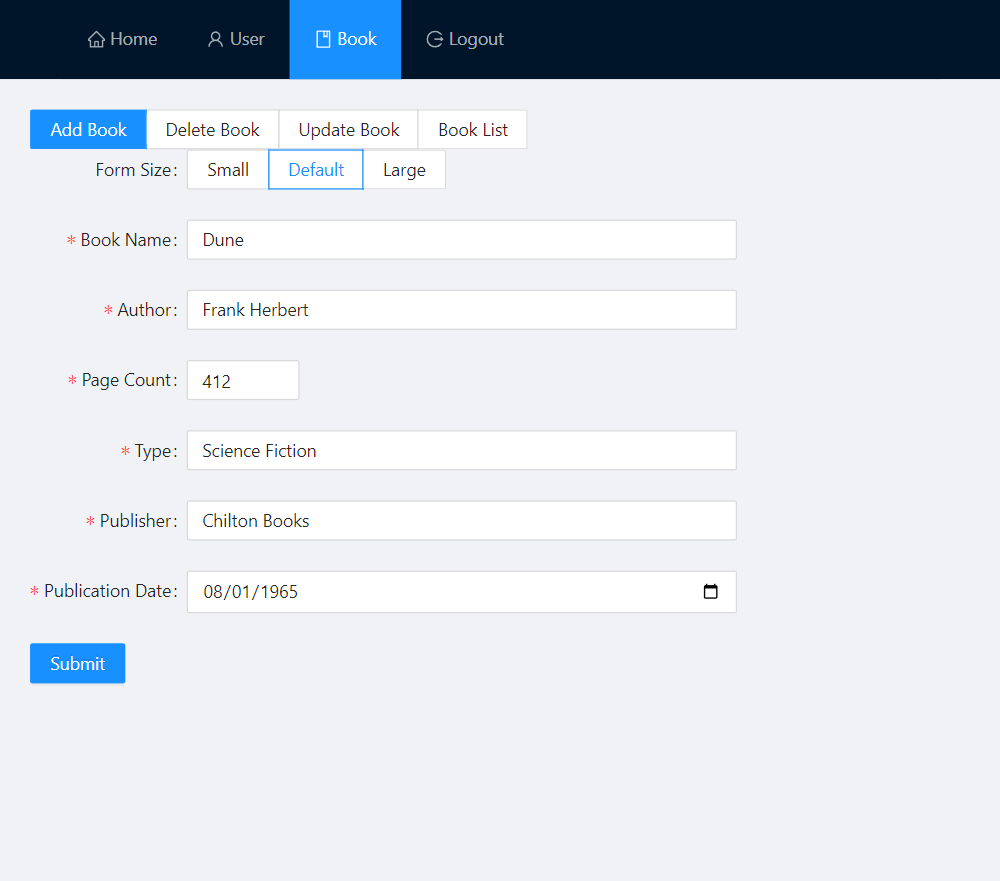
\includegraphics[width=\linewidth]{img/front-end/add-book-form.png}
    \caption{Book Adding Form}
  \end{figure}
\end{minipage}
\begin{minipage}{.49\textwidth}
  \begin{figure}[H]
    \centering
    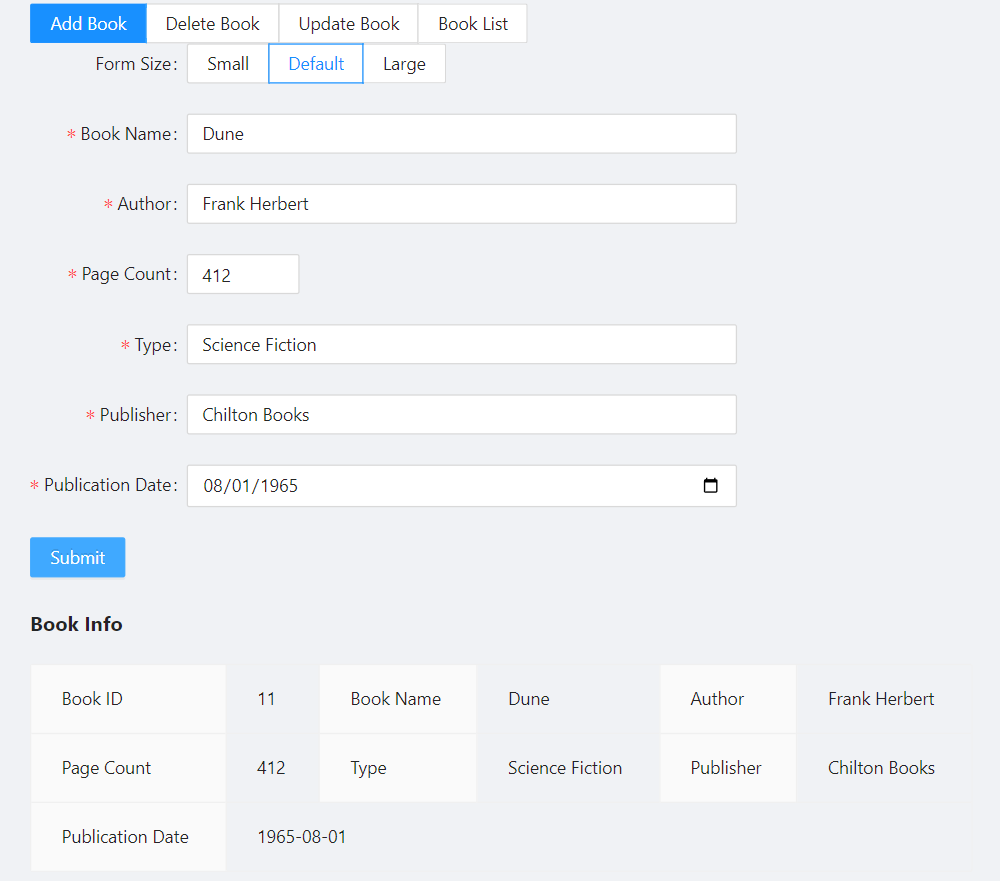
\includegraphics[width=\linewidth]{img/front-end/add-book-added.png}
    \caption{Book Added to Database}
  \end{figure}
\end{minipage}

\subsection{\texttt{Delete and Update Book}}

The \texttt{Delete} and \texttt{Update} pages of the book are similar to user's and special to admins. Both pages support searching books by both id and username, and searching option can be changed by using the radio buttons. Again, when the input area is cleared, page is updated and user data is resetted. Both pages also support the pagination and pagination setting changes. Admin can change the pagination setting by using the navigation below. Additionally, in both pages, admin can see the information of the books.

The only difference between \texttt{Delete Book} and \texttt{Delete User} is the visualizing data. I preffered the `Descriptions' of antd to visualize the data of a book. The differences between \texttt{Update Book} and \texttt{Update User} are the visualizing method and updating form. Only page count, publisher, or publication date of a book can be updated.

\begin{minipage}{.49\textwidth}
  \begin{figure}[H]
    \centering
    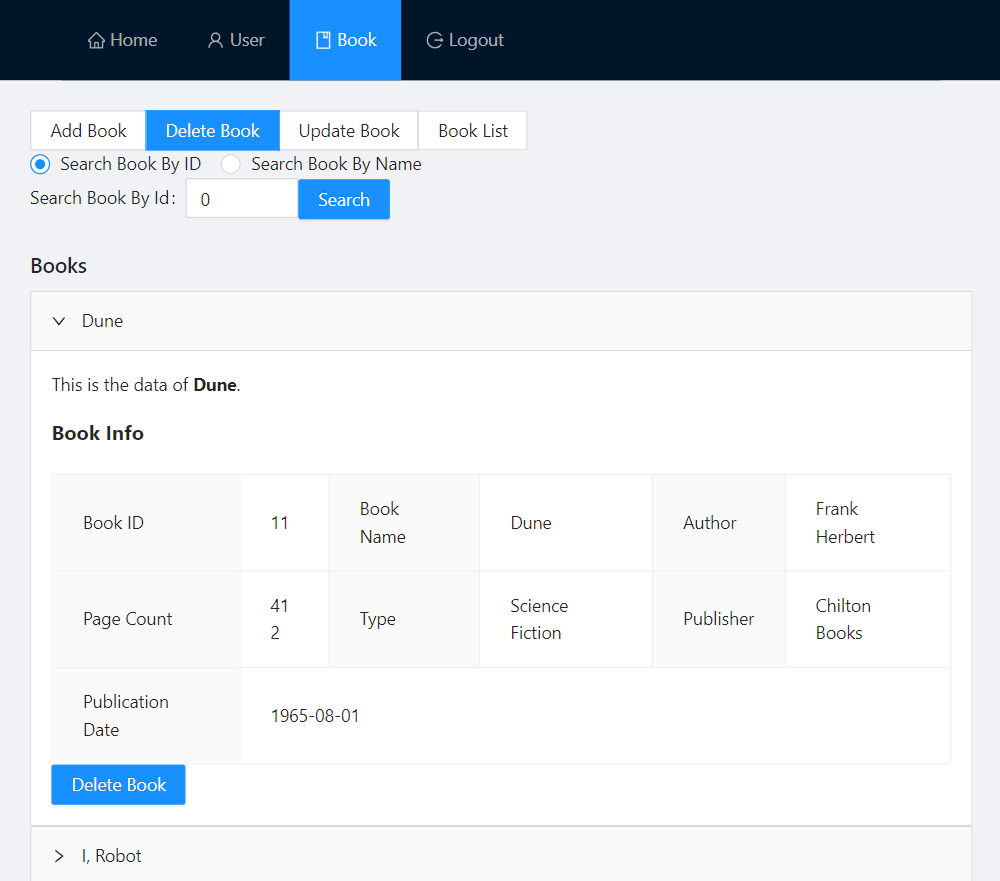
\includegraphics[width=\linewidth]{img/front-end/book-delete.png}
    \caption{Book Delete}
  \end{figure}
\end{minipage}
\begin{minipage}{.49\textwidth}
  \begin{figure}[H]
    \centering
    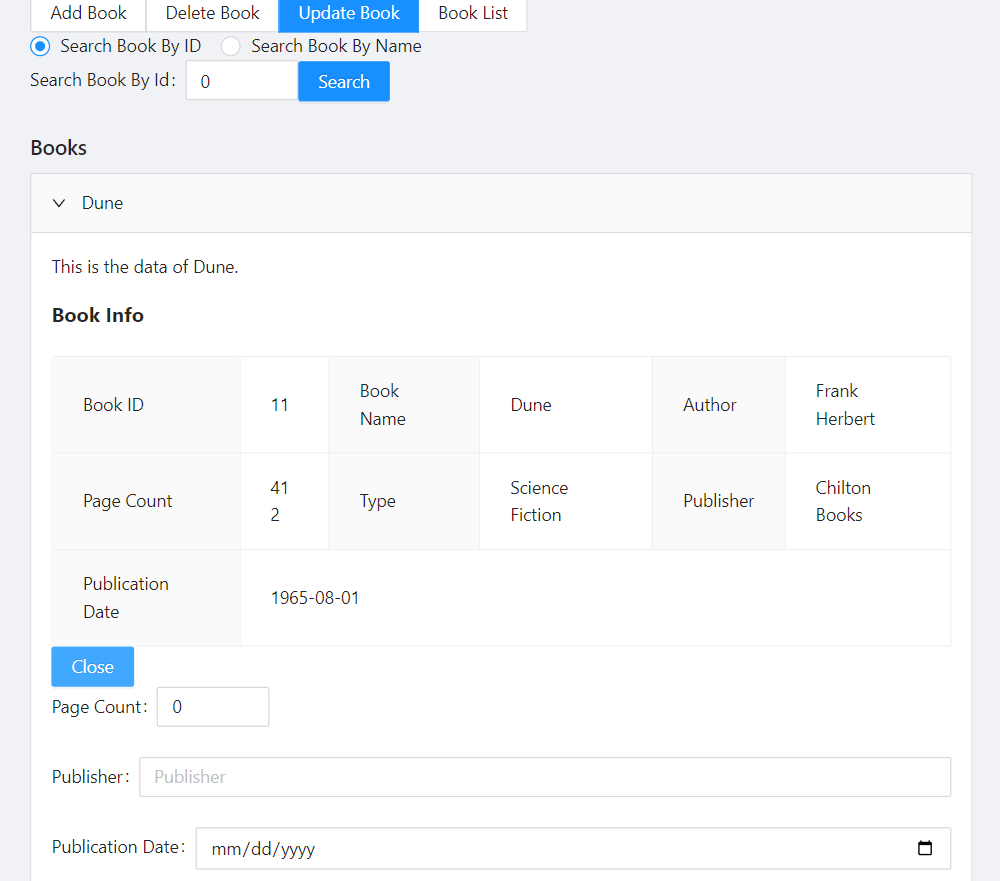
\includegraphics[width=\linewidth]{img/front-end/book-update.png}
    \caption{Book Update}
  \end{figure}
\end{minipage}

\subsection{\texttt{Book List}}

This page is accessible by all users, and the default rendered page of \texttt{Book} item. `Table' and `Pagination' of antd are used in this page and it lists all the books in database and provides searching by both id and name. In each row, information of each book is provided as well as the actions which are operated on the book in that row. Any user can add or remove the book to/from his/her read or favorite lists.

\begin{minipage}{.49\textwidth}
  \begin{figure}[H]
    \centering
    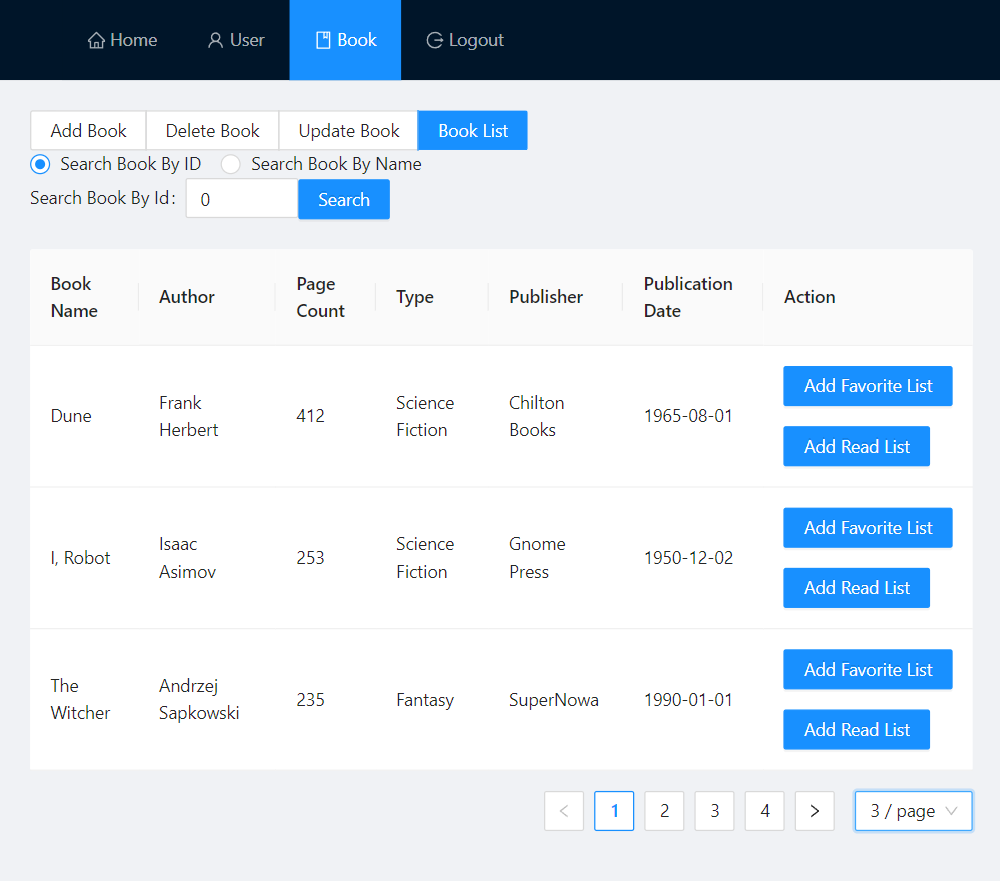
\includegraphics[width=\linewidth]{img/front-end/book-list.png}
    \caption{Book List}
  \end{figure}
\end{minipage}
\begin{minipage}{.49\textwidth}
  \begin{figure}[H]
    \centering
    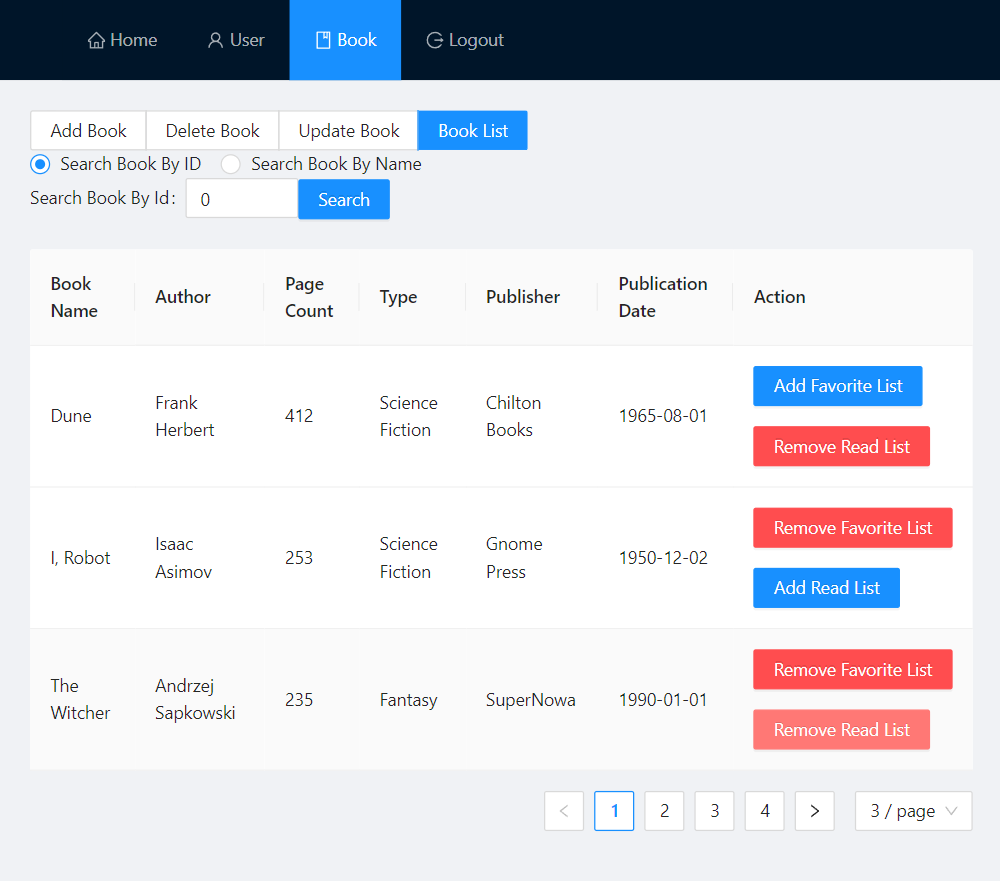
\includegraphics[width=\linewidth]{img/front-end/book-list-example.png}
    \caption{Book List Example}
  \end{figure}
\end{minipage}

If the book is not added to related list, the action button is blue and the text of it specifies the adding operation. However, if the book is already added to related list, the action button is red and the text of it specifies the removing operation. When the button is clicked a request is sent to database and the state of the book data is updated. As a result of that, page is re-rendered with the new state.

This part was hard to code. Putting the action buttons and performing their operations were more difficult, aside from the force of the table. It was easy to send a request and saving the book to user's list at database; however, it was hard to update and re-render the book data and the state of book. I thought to do this task without new getting request because of the complexity. Also, at the first place, the book information had problem when the pagination is updated. To solve these problems, I spent several hours.

